% Per effetuare l'esame orale di discussione del progetto, è OBBLIGATORIO caricare le slide (minimo 4, massimo 7) in PDF che descrivono il progetto.
%Le slide DEVONO essere strutturate in questo modo:
%almeno 1 (massimo 2) slide per descrivere le funzionalità
%1 slide per descrivere le tencnologie (es. BLE, qrcode reader, camera, sensori biometrici, open data esterni, API per servizi di mappe, ecc.) -- basta un elenco puntato
%almeno 2 (massimo 4) slide con gli screeshot dell'applicazione

\documentclass[10pt]{beamer}
\usepackage[utf8]{inputenc}
\usepackage{graphicx}
\usepackage{multicol}
\usepackage {mathtools}
\usetheme{CambridgeUS}
\usecolortheme{dolphin}

% set colors
\definecolor{myNewColorA}{RGB}{0, 55, 158}
\definecolor{myNewColorB}{RGB}{0, 55, 158}
\definecolor{myNewColorC}{RGB}{0, 55, 158}
\setbeamercolor*{palette primary}{bg=myNewColorC, fg = white}
\setbeamercolor*{palette secondary}{bg=myNewColorB, fg = white}
\setbeamercolor*{palette tertiary}{bg=myNewColorA, fg = white}
\setbeamercolor*{titlelike}{fg=myNewColorA}
\setbeamercolor*{title}{bg=myNewColorA, fg = white}
\setbeamercolor*{item}{fg=myNewColorA}
\setbeamercolor*{caption name}{fg=myNewColorA}
\usefonttheme{professionalfonts}
\usepackage{natbib}
\usepackage{hyperref}
%------------------------------------------------------------
\titlegraphic{
\includegraphics[height=1.5cm]{Screenshot 2022-09-15 at 21.36.06.png}} 

\setbeamerfont{title}{size=\large}
\setbeamerfont{subtitle}{size=\small}
\setbeamerfont{author}{size=\small}
\setbeamerfont{date}{size=\small}
\setbeamerfont{institute}{size=\small}
\title[MaggioliEbook]{MaggioliEbook \\ Digital Publishing E-Reader Mobile App}

\institute[0000926989]{Alma Mater Studiorum - Università di Bologna \\ Campus di Cesena \\ Programmazione di Sistemi Mobile}
\author[Filippo Paganelli]{Filippo Paganelli \\ 0000926989 \\ filippo.paganelli3@studio.unibo.it}
\date[\textcolor{white}{A.A. 21/22} ]
{A.A. 21/22}

%------------------------------------------------------------
%This block of commands puts the table of contents at the 
%beginning of each section and highlights the current section:
%\AtBeginSection[]
%{
%  \begin{frame}
%    \frametitle{Contents}
%    \tableofcontents[currentsection]
%  \end{frame}
%}
%\AtBeginSection[]{
%  \begin{frame}
%  \vfill
%  \centering
%  \begin{beamercolorbox}[sep=8pt,center,shadow=true,rounded=true]{title}
%    \usebeamerfont{title}\insertsectionhead\par%
%  \end{beamercolorbox}
%  \vfill
%  \end{frame}
%}
%------------------------------------------------------------

\begin{document}

%The next statement creates the title page.
\frame{\titlepage}
\begin{frame}
\frametitle{Contents}
\tableofcontents
\end{frame}
%------------------------------------------------------------
\section{Funzionalità}
    \begin{frame}{Funzionalità}
     \begin{itemize}
         \item Lettura dei contenuti digitali forniti da Maggioli.
         \item I contenuti sono visualizzati in modo fluido, adattandosi alle dimensioni del dispositivo e alle necessità dell'utente (grandezza caratteri, margini, spacing, tema chiaro/sepia/scuro, contrasto, ...).
         \item I contenuti che è possibile visualizzare sono basati sugli abbonamenti sottoscritti dall'utente.
         \item Accesso tramite autenticazione.
         \item Gestione preferiti, evidenziazione, sottolineatura, annotazioni e segnalibri.
         \item Ricerca testuale all'interno del contenuto.
     \end{itemize}
    \end{frame}

\section{Tecnologie}
\begin{frame}{Tecnologie}
    \begin{itemize}
    \item \textbf{SDK \& Tools}
    \begin{itemize}
        \item \href{https://developer.android.com/about/versions/12}{\textit{Android} 12 (API 31, 32)} + \href{https://github.com/JetBrains/kotlin/releases/tag/v1.7.0}{\textit{Kotlin} 1.7.0}
        \item \href{https://docs.gradle.org/7.4/userguide/userguide.html}{\textit{Gradle} 7.4}
    \end{itemize}
    \item \textbf{Architettura}
    \begin{itemize}
        \item \href{https://kotlinlang.org/lp/mobile/}{\textit{Kotlin Multiplatform}}
        \item \href{https://developer.android.com/guide/navigation/navigation-migrate}{\textit{Single Activity}}
        \item \href{https://developer.android.com/jetpack}{Android Jetpack} - \textit{View Model + Flow +  Repository}, \href{https://developer.android.com/jetpack/compose}{\textit{Compose}}, \href{https://developer.android.com/guide/navigation}{\textit{Navigation}}, \href{https://developer.android.com/topic/libraries/architecture/paging/v3-overview}{Paging 3}
    \end{itemize}
    \item \textbf{Librerie}
    \begin{itemize}
         \item \href{https://insert-koin.io/}{\textit{Koin}} - Dependency Injection
         \item \href{https://cashapp.github.io/sqldelight/}{\textit{SqlDelight}} - Storage (astrazione SQLite)
         \item \href{https://ktor.io/}{\textit{Ktor}} - Networking (Http Client)
         \item \href{https://github.com/AAkira/Napier}{\textit{Napier}} - Logging
         \item \href{https://github.com/Liftric/KVault}{\textit{KVault}} - Storage (SharedPreferences)
         \item \href{https://readium.org/}{\textit{Readium}} - Lettore EPUB
    \end{itemize}
     \end{itemize}
\end{frame}

\section{Screenshots}
    \begin{frame}{Screenshots}
        \begin{multicols}{3}
            \begin{figure}[H]
                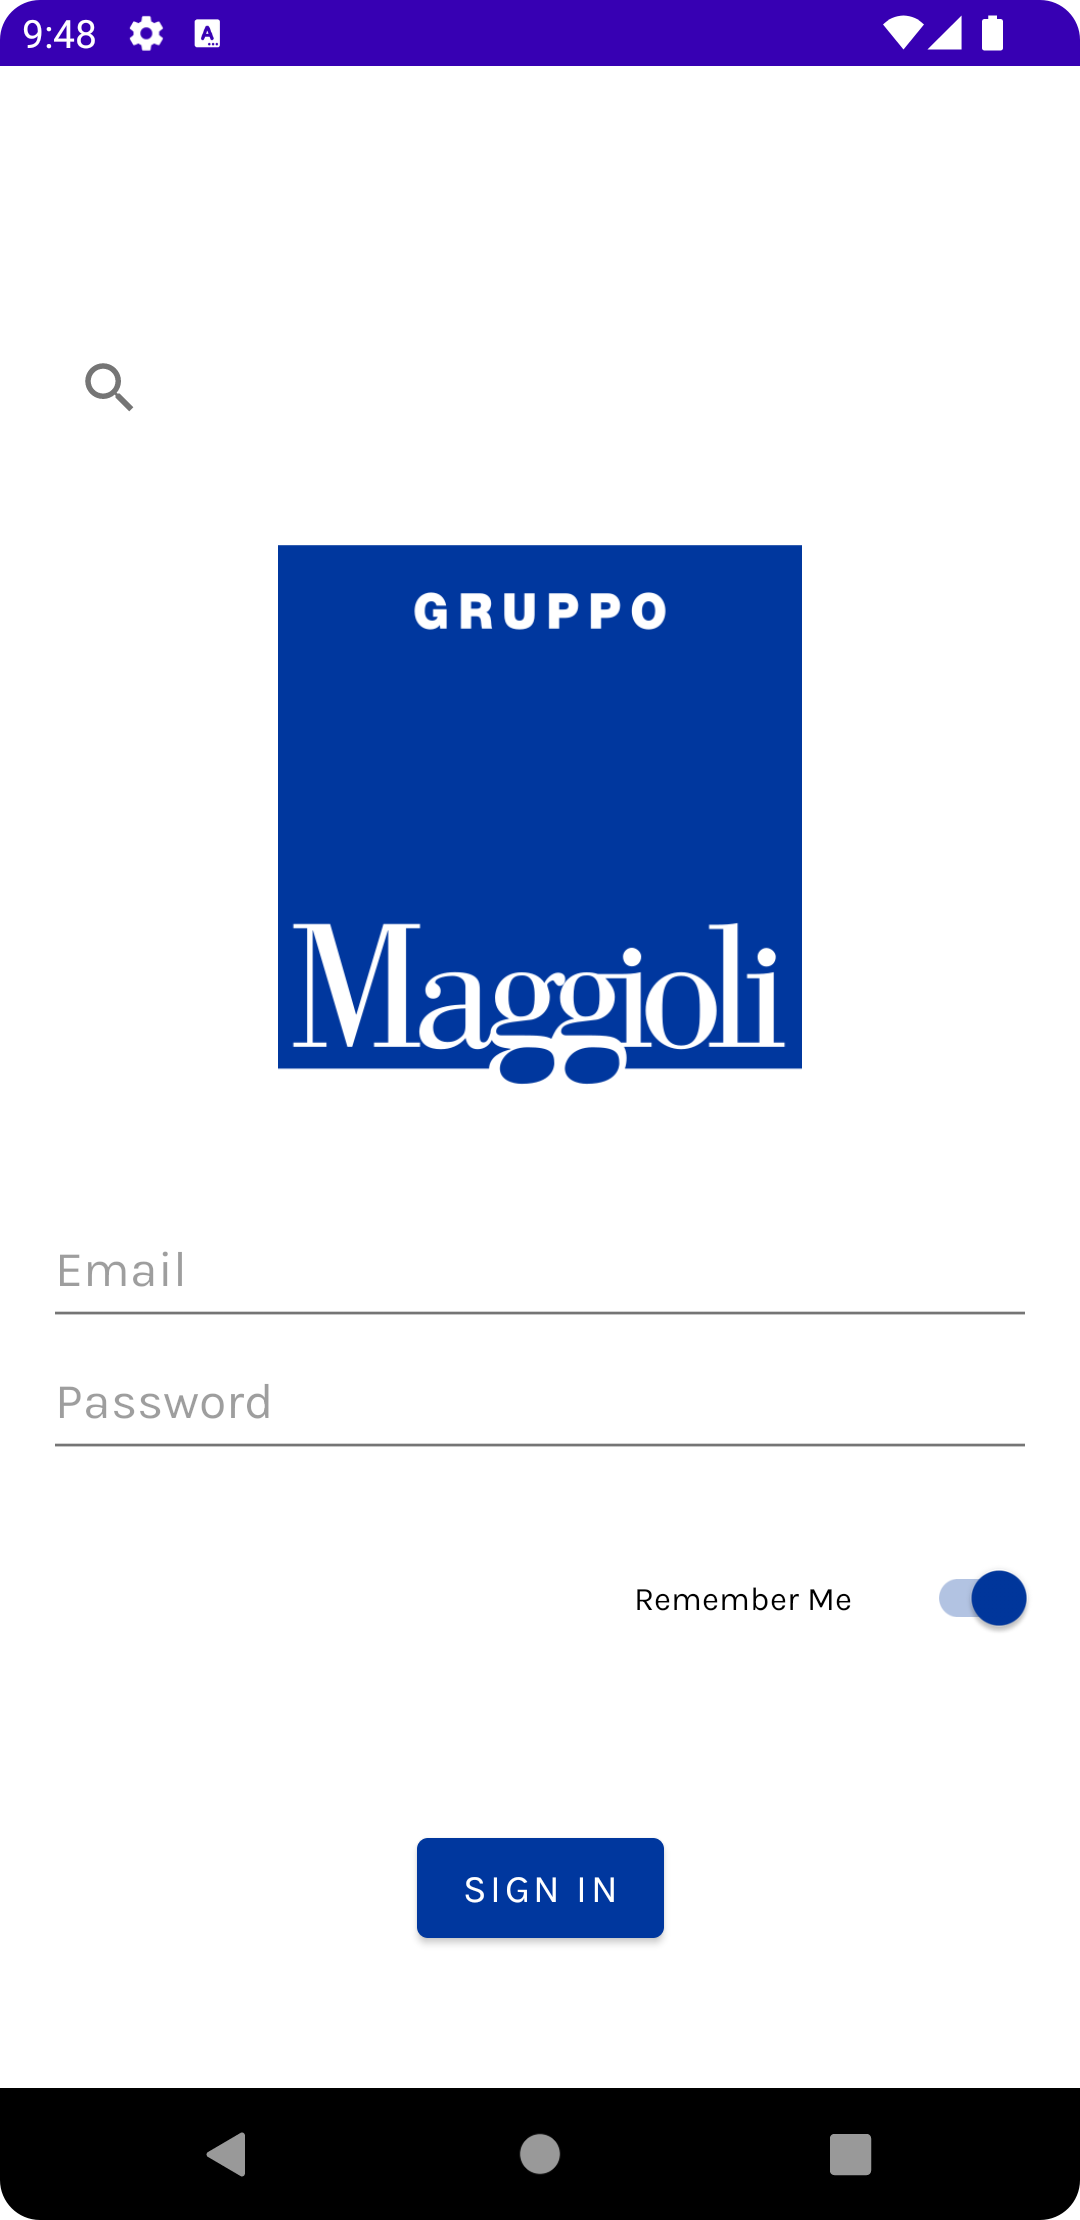
\includegraphics[width=0.2\textwidth]{login.png}
                \caption{Schermata di login degli utenti abbonati}
                \label{login}
            \end{figure}
            
            \begin{figure}[H]
                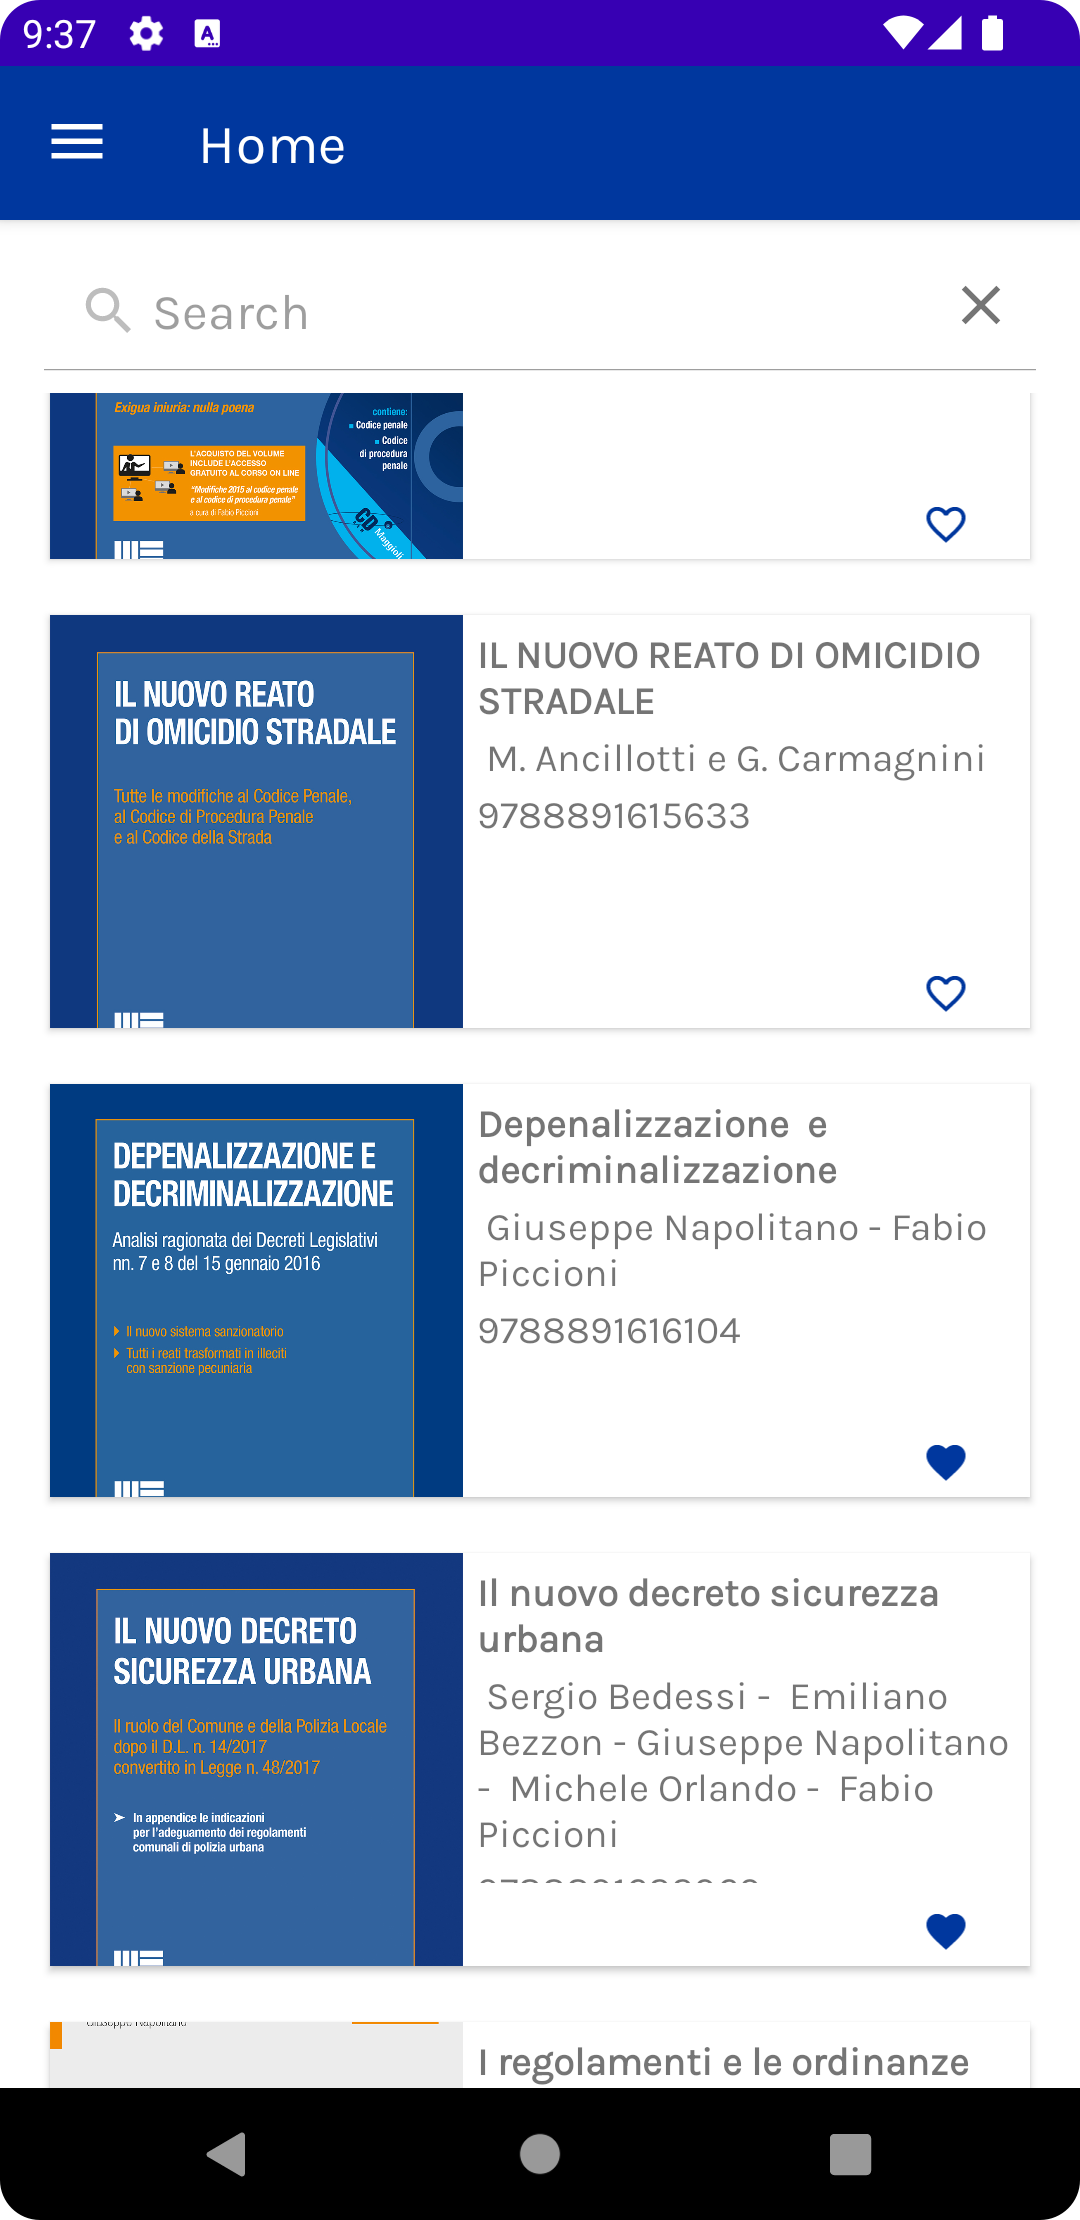
\includegraphics[width=0.2\textwidth]{home.png}
                \caption{Schermata home principale per la visualizzazione e la ricerca dei documenti digitali Maggioli}
                \label{home}
            \end{figure}
            
            \begin{figure}[H]
                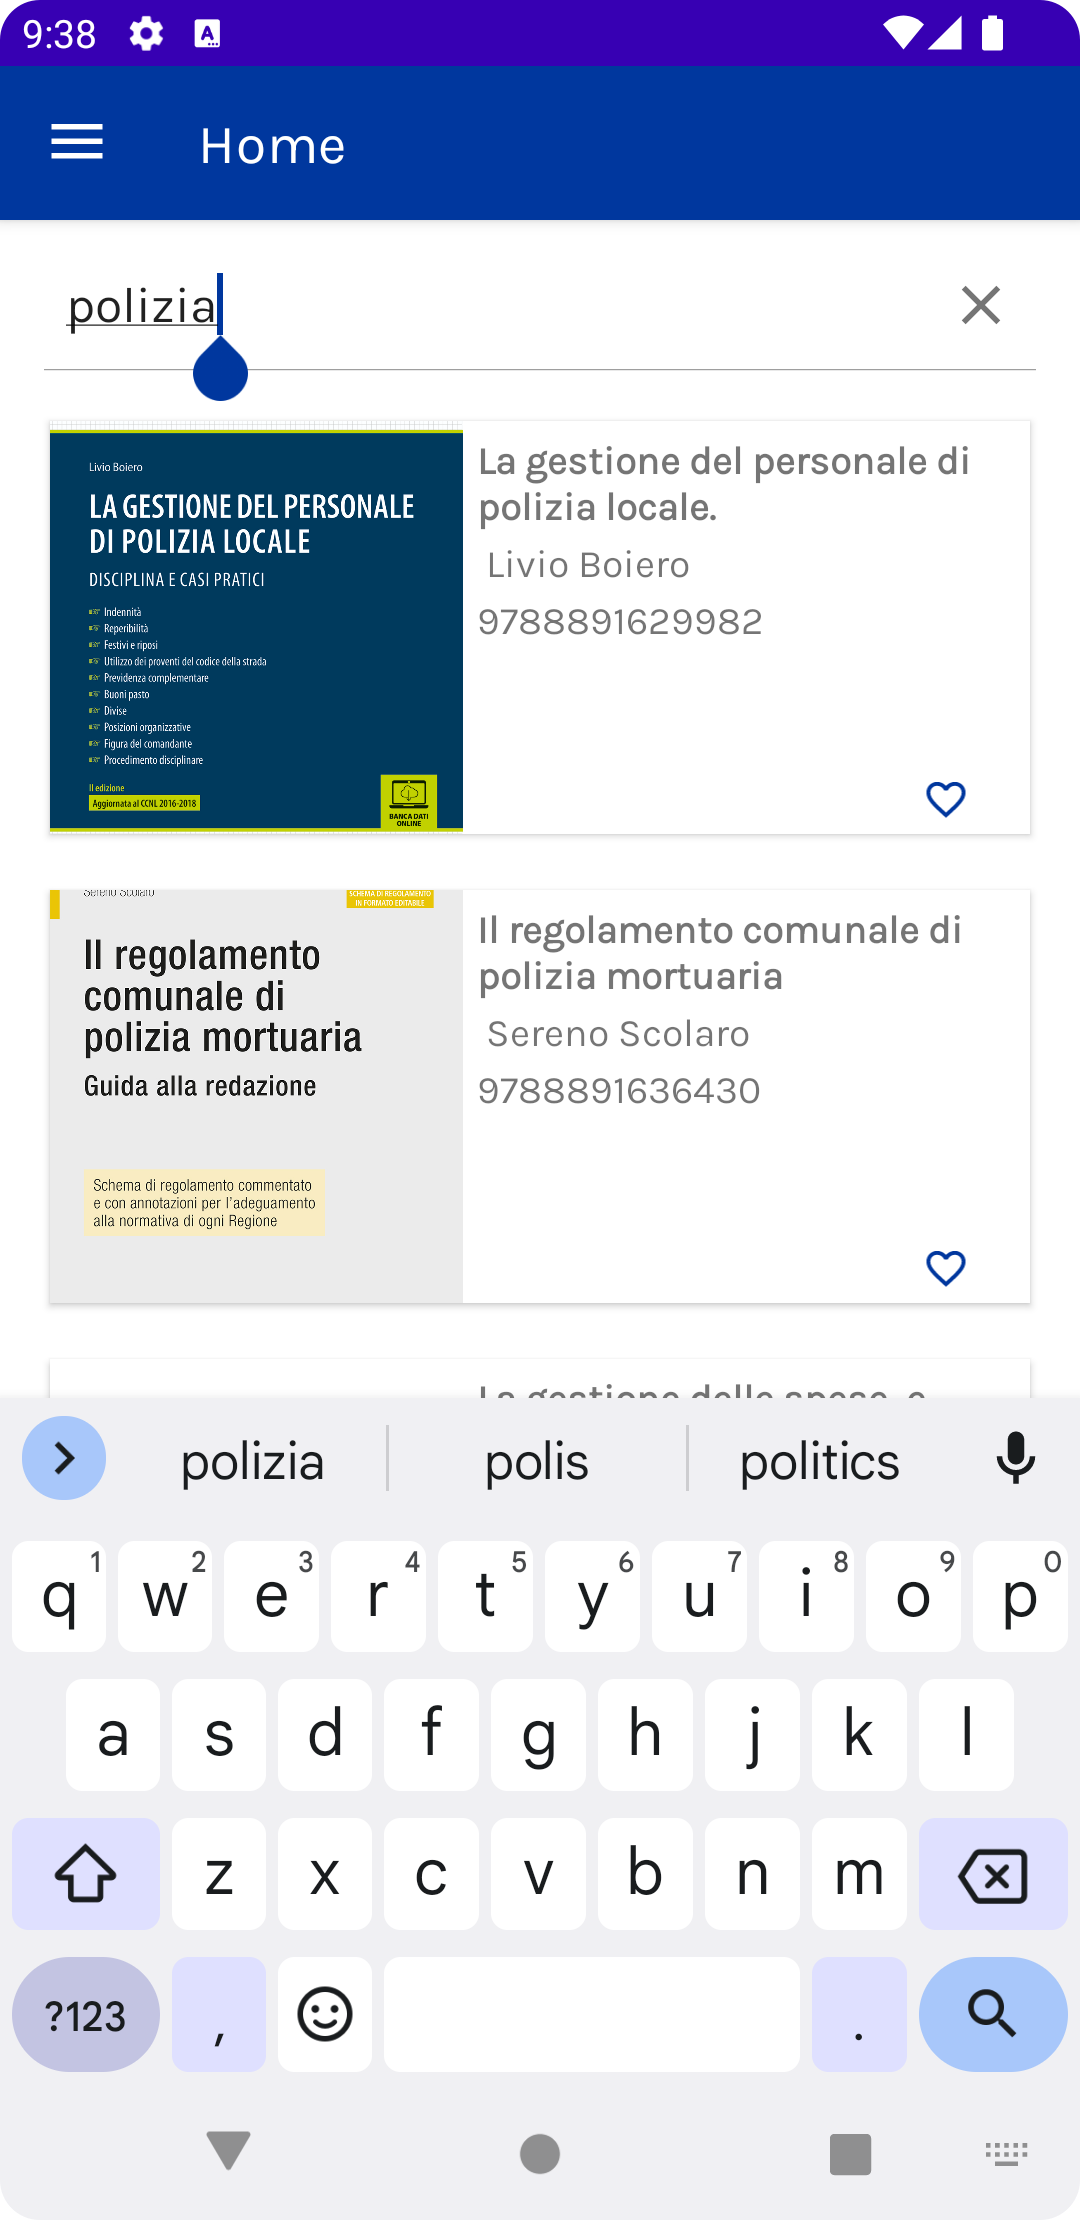
\includegraphics[width=0.2\textwidth]{ricerca.png}
                \caption{Esempio di ricerca per parola chiave nella schermata principale}
                \label{ricerca}
            \end{figure}
        \end{multicols}
    \end{frame}

    \begin{frame}{Screenshots}
        \begin{multicols}{3}
            \begin{figure}[H]
                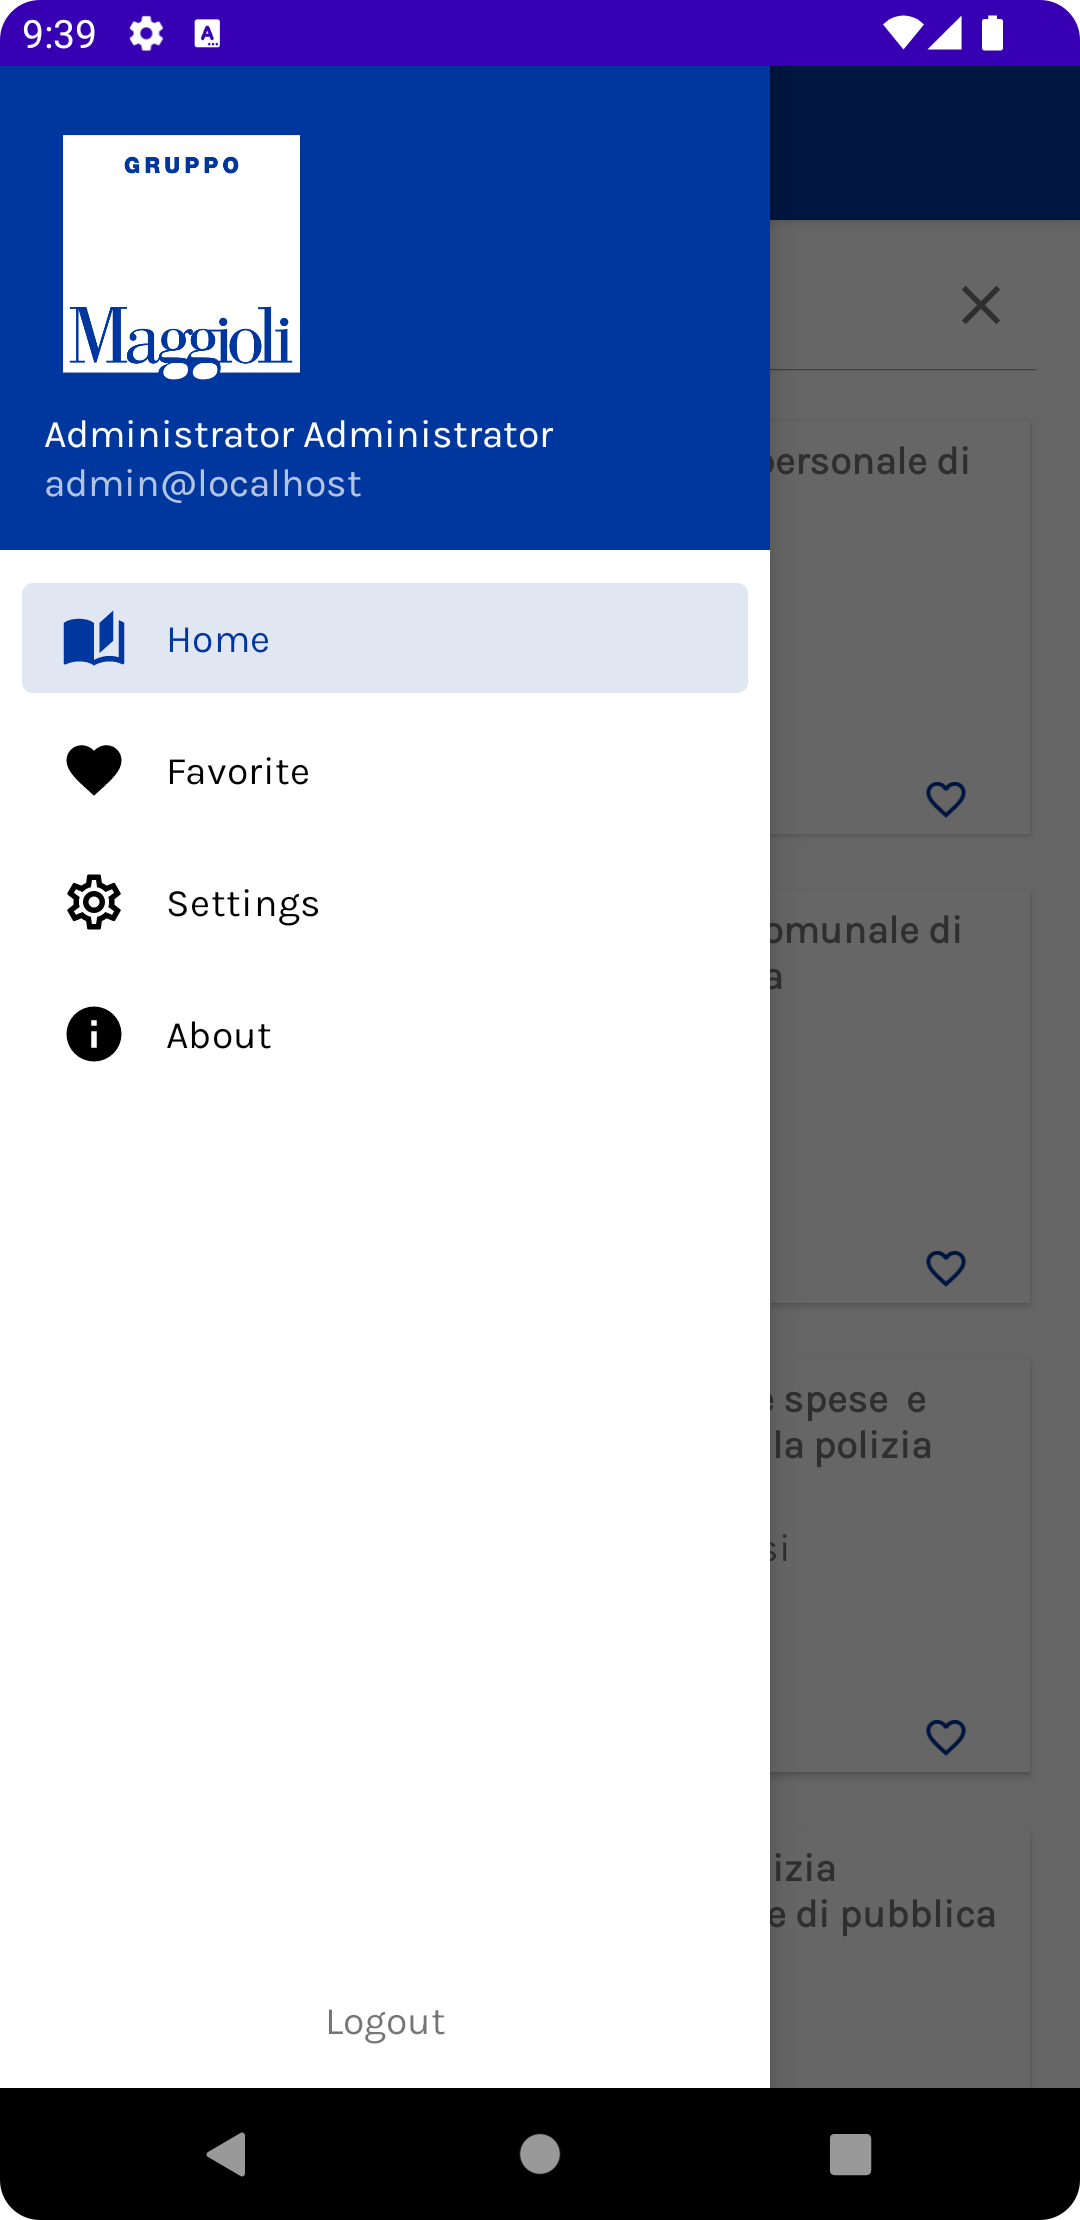
\includegraphics[width=0.2\textwidth]{sidenav.png}
                \caption{Menu laterale per la navigazione all'interno della applicazione}
                \label{sidenav}
            \end{figure}
            
            \begin{figure}[H]
                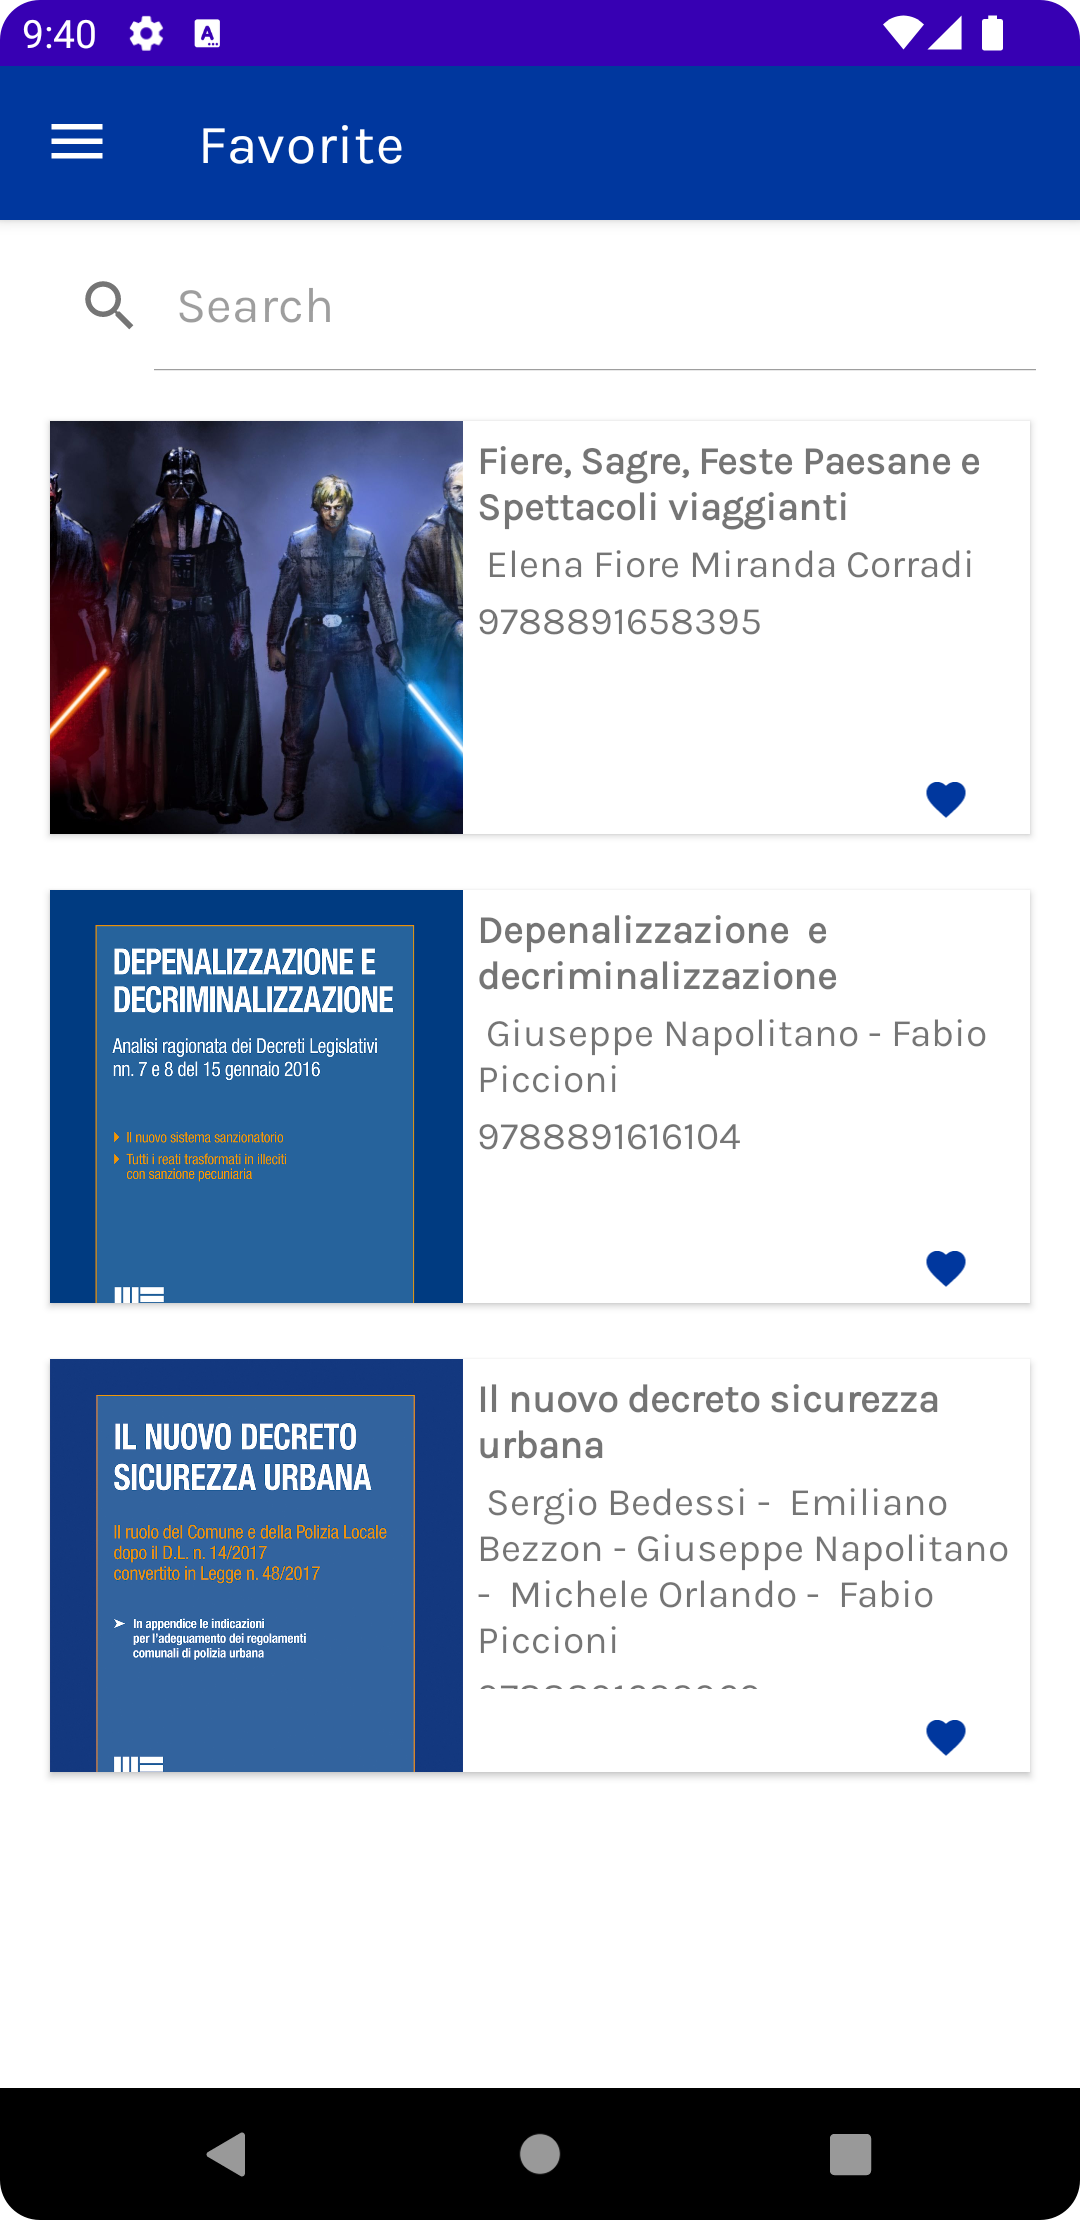
\includegraphics[width=0.2\textwidth]{preferiti.png}
                \caption{Schermata per la visualizzazione e la ricerca dei documenti preferiti dall'utente}
                \label{preferiti}
            \end{figure}

            \begin{figure}[H]
                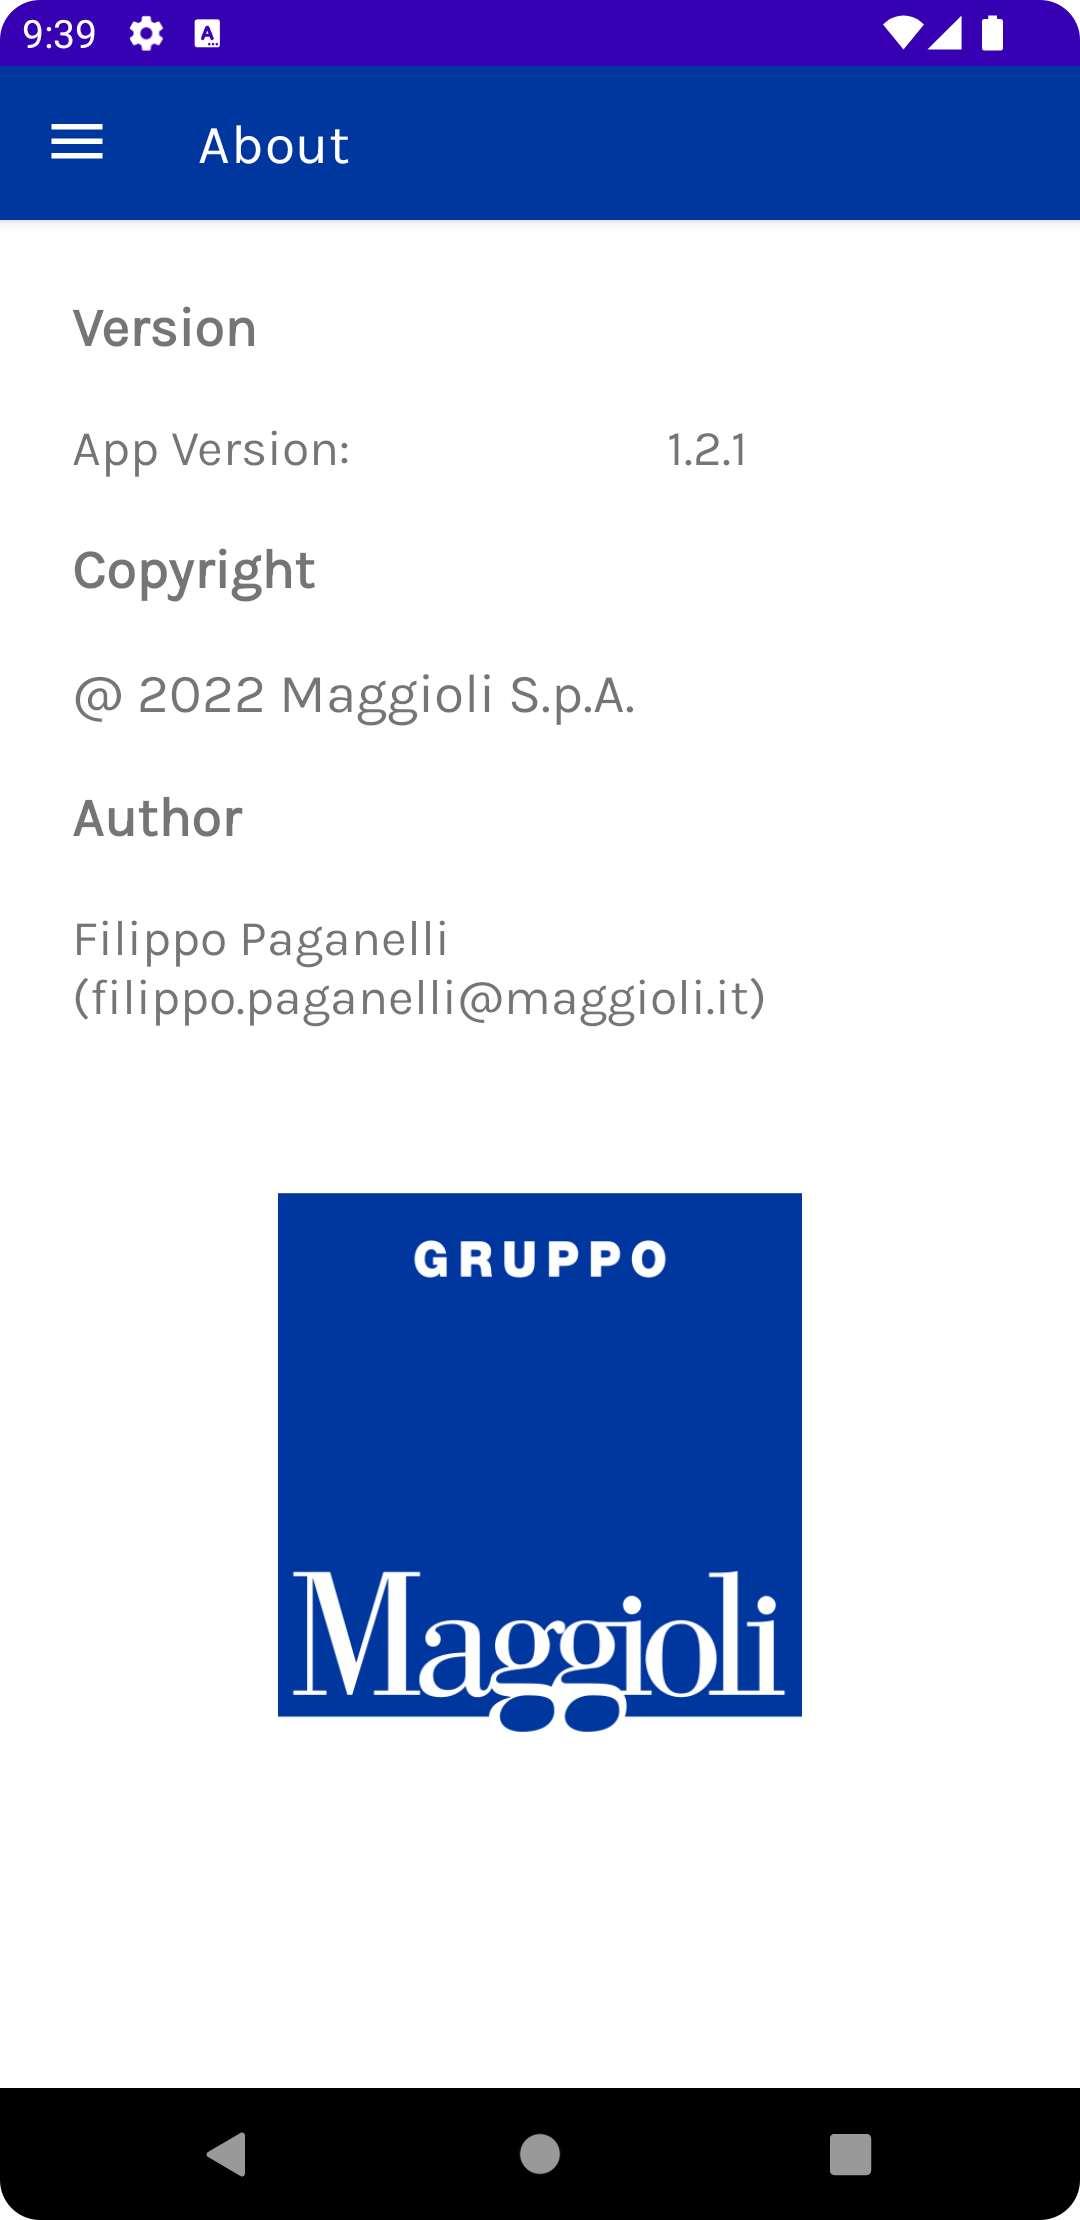
\includegraphics[width=0.2\textwidth]{about.png}
                \caption{Schermata per la visualizzazione delle informazioni generali relative alla applicazione}
                \label{about}
            \end{figure}
        \end{multicols}
    \end{frame}

    \begin{frame}{Screenshots}
        \begin{multicols}{3}
            \begin{figure}[H]
                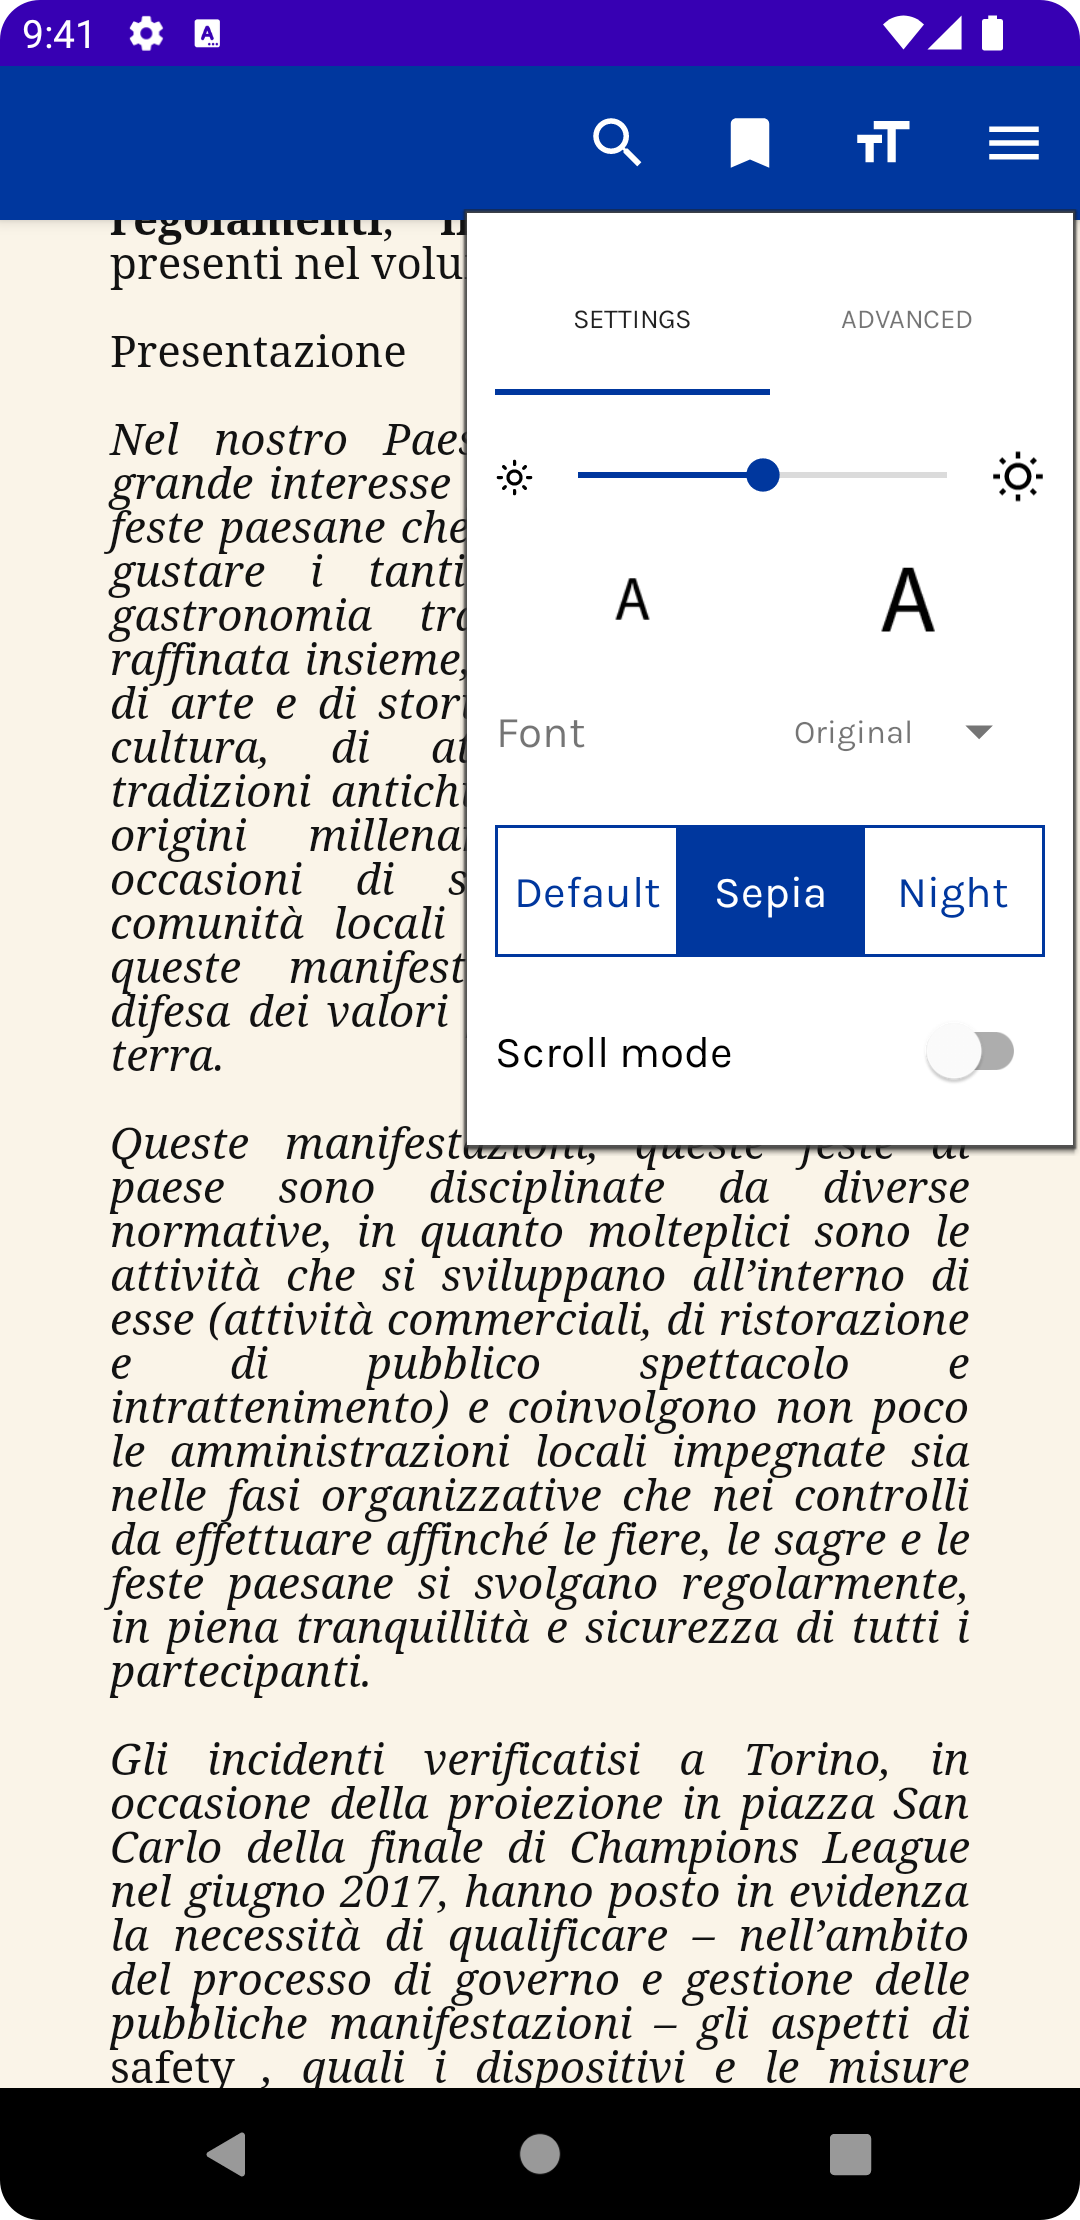
\includegraphics[width=0.2\textwidth]{reader_settings.png}
                \caption{Lettura documento digitale d'esempio e impostazioni del lettore}
                \label{reader}
            \end{figure}
            
            \begin{figure}[H]
                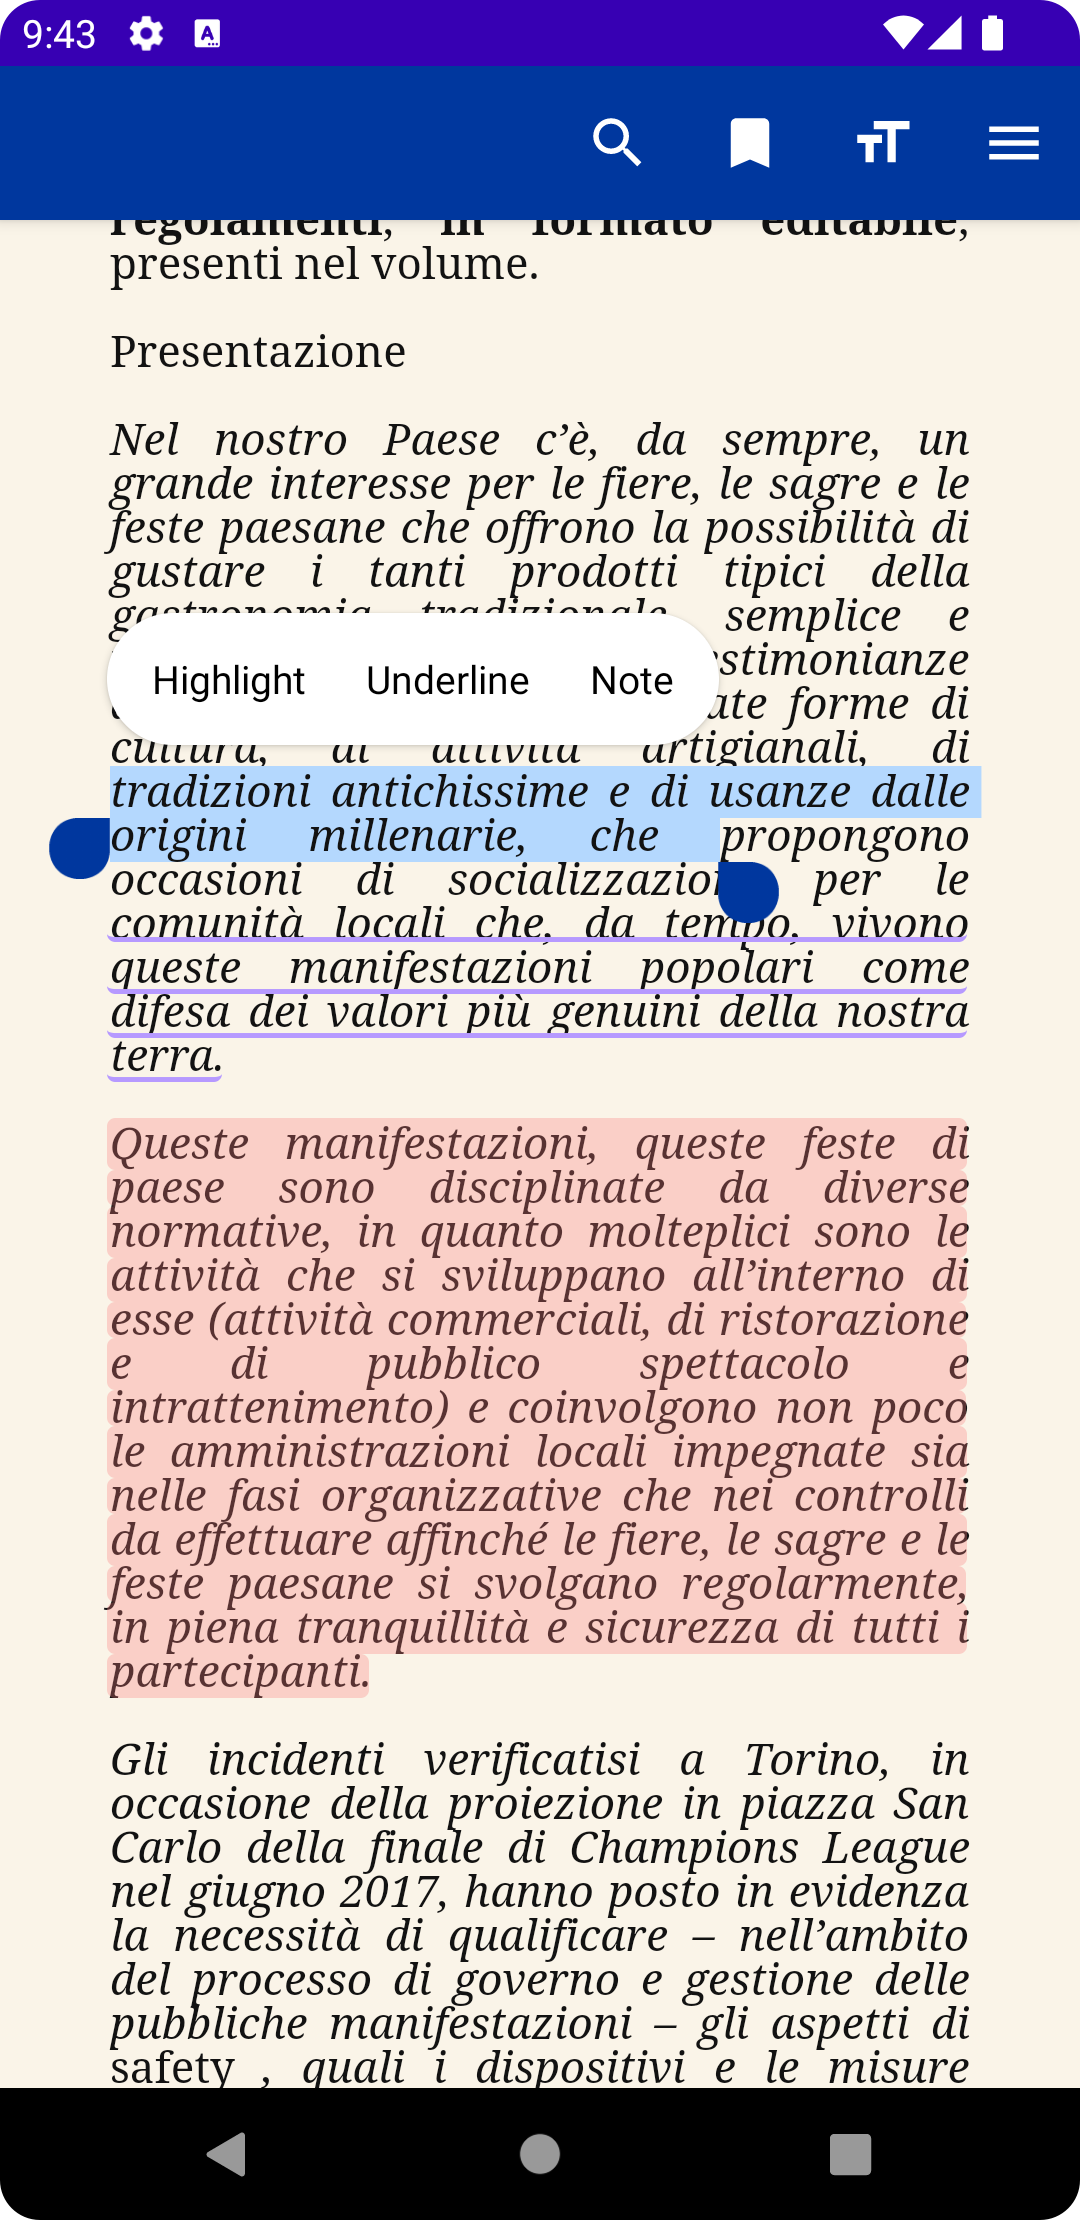
\includegraphics[width=0.2\textwidth]{annotations.png}
                \caption{Esempio di inserimento di annotazioni come evidenziazioni e sottolineature}
                \label{annotations}
            \end{figure}
            
            \begin{figure}[H]
                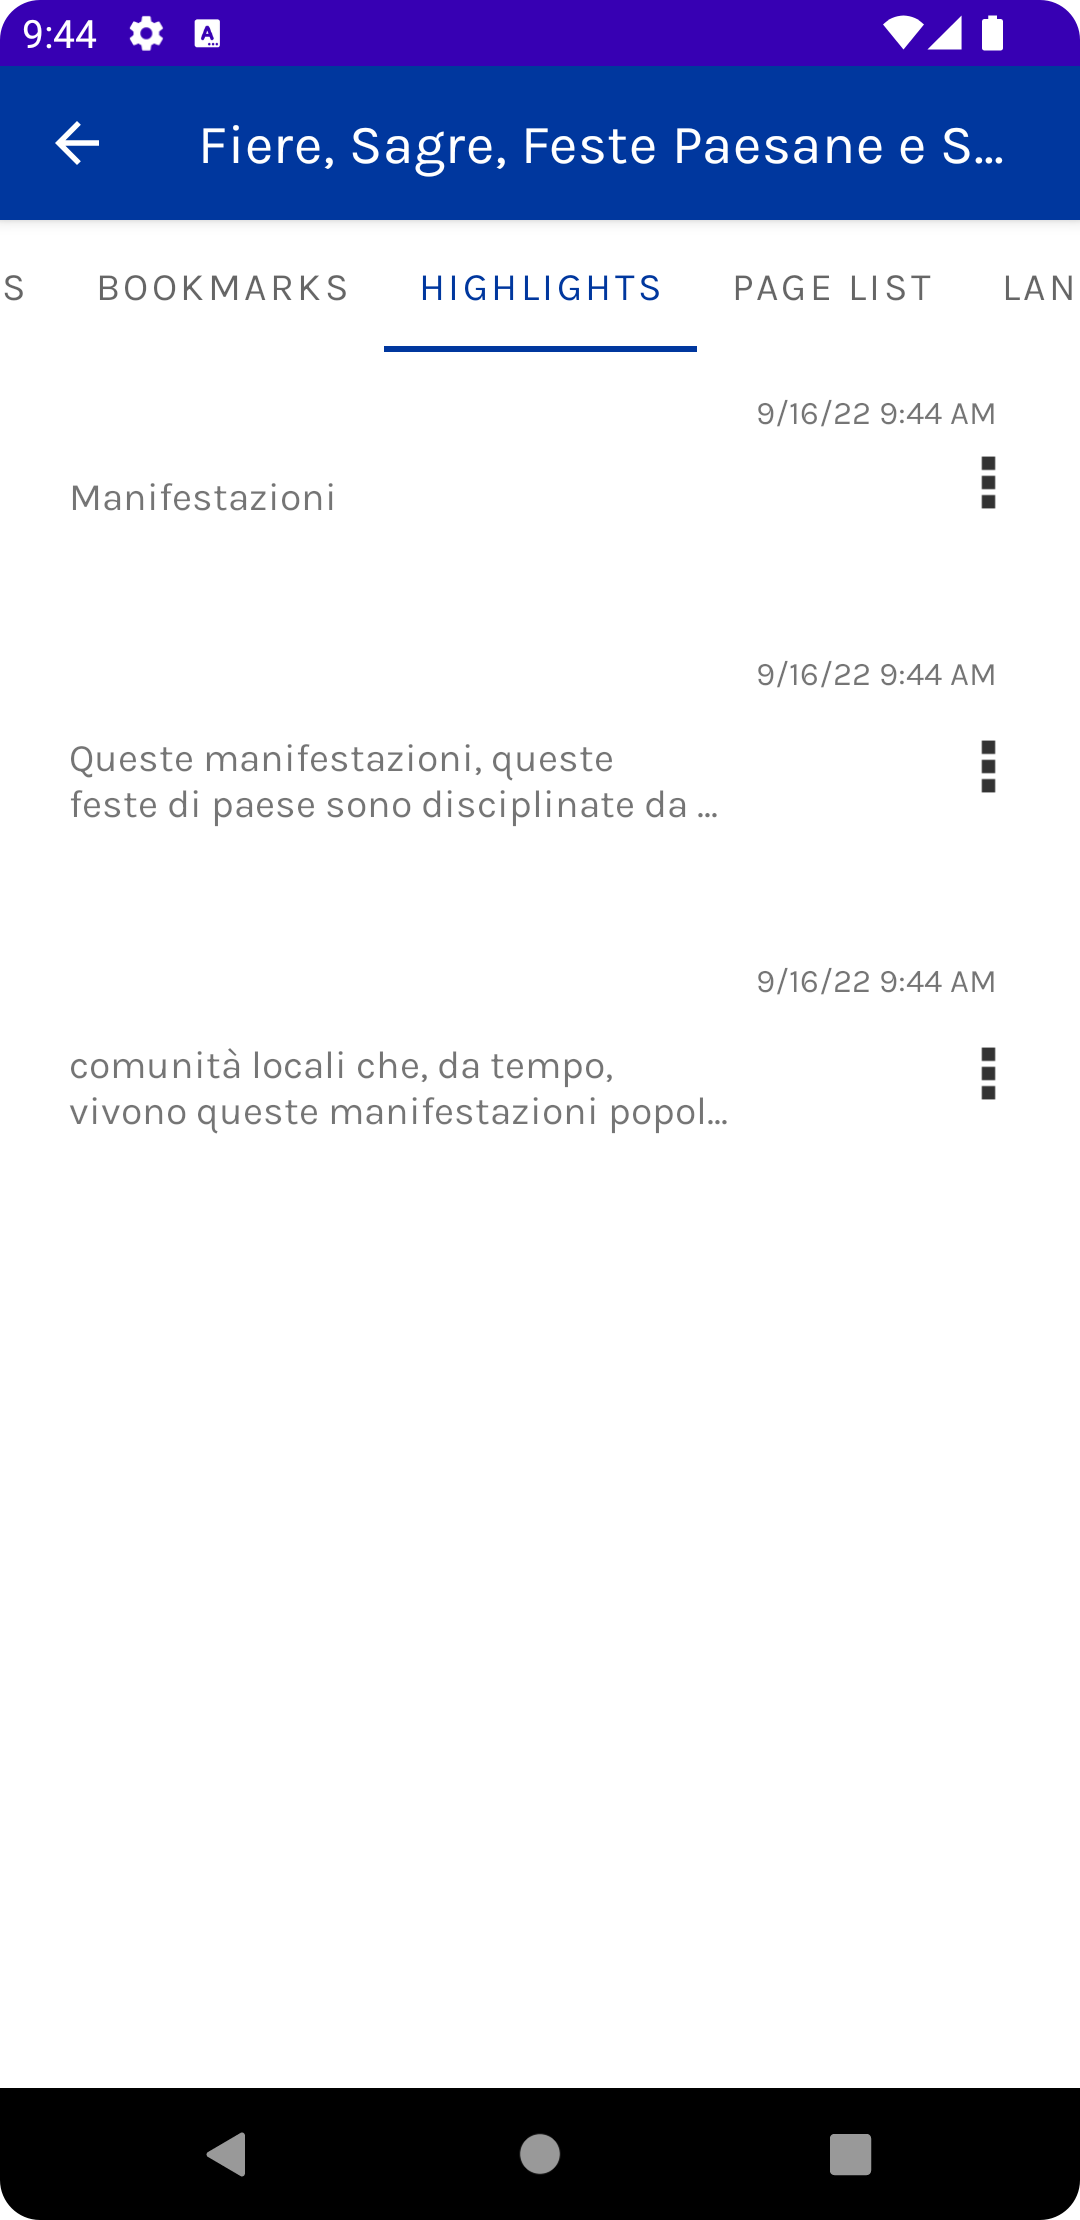
\includegraphics[width=0.2\textwidth]{annotation2.png}
                \caption{Annotazioni memorizzate sul dispositivo e consultabili dal menu del lettore}
                \label{annotation2}
            \end{figure}
        \end{multicols}
    \end{frame}

    \begin{frame}{Screenshots}
        \begin{multicols}{3}
            \begin{figure}[H]
                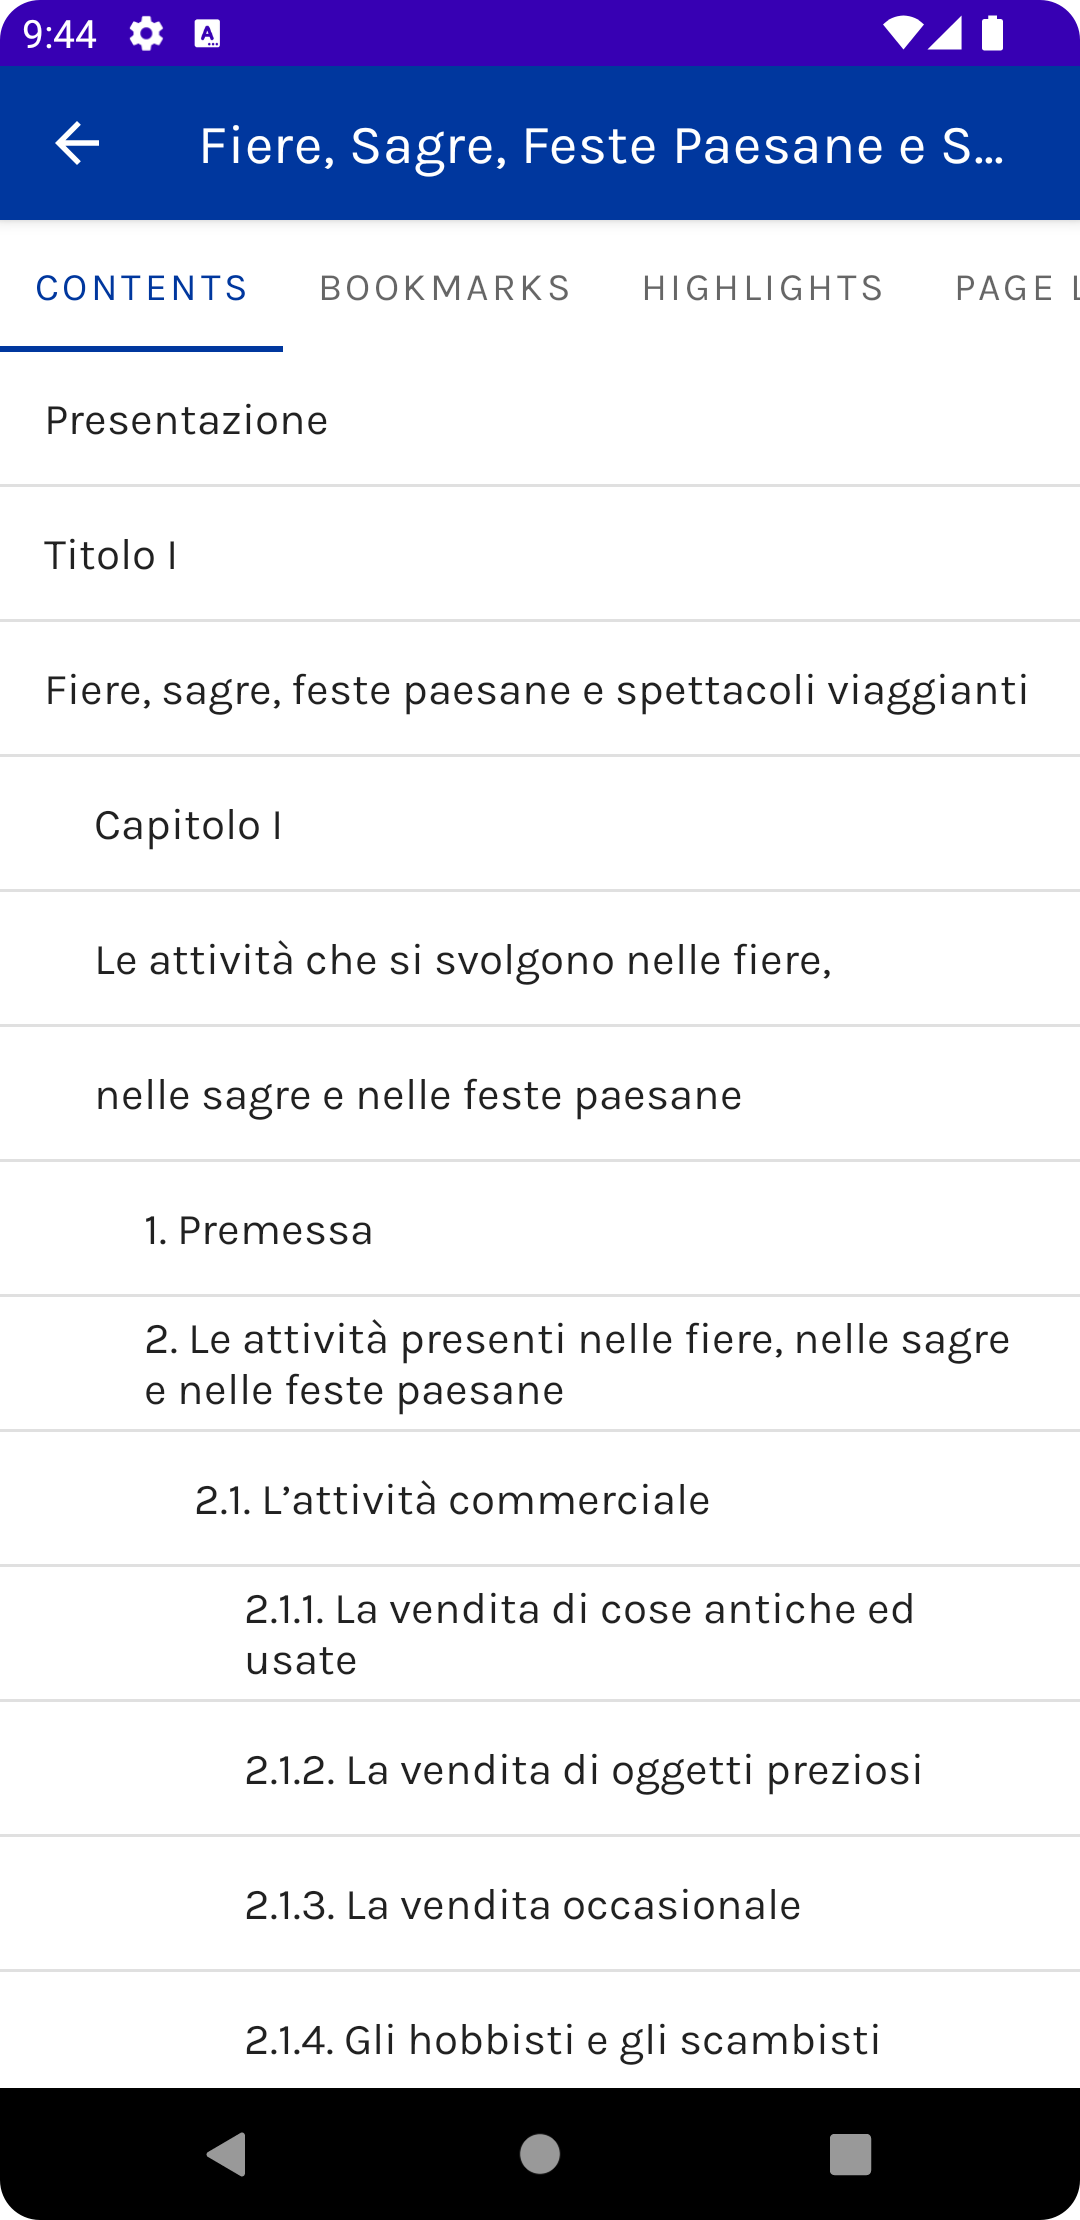
\includegraphics[width=0.2\textwidth]{toc.png}
                \caption{Elenco dei contenuti (TOC) del documento aperto e consultabile dal menu del lettore}
                \label{toc}
            \end{figure}
            
            \begin{figure}[H]
                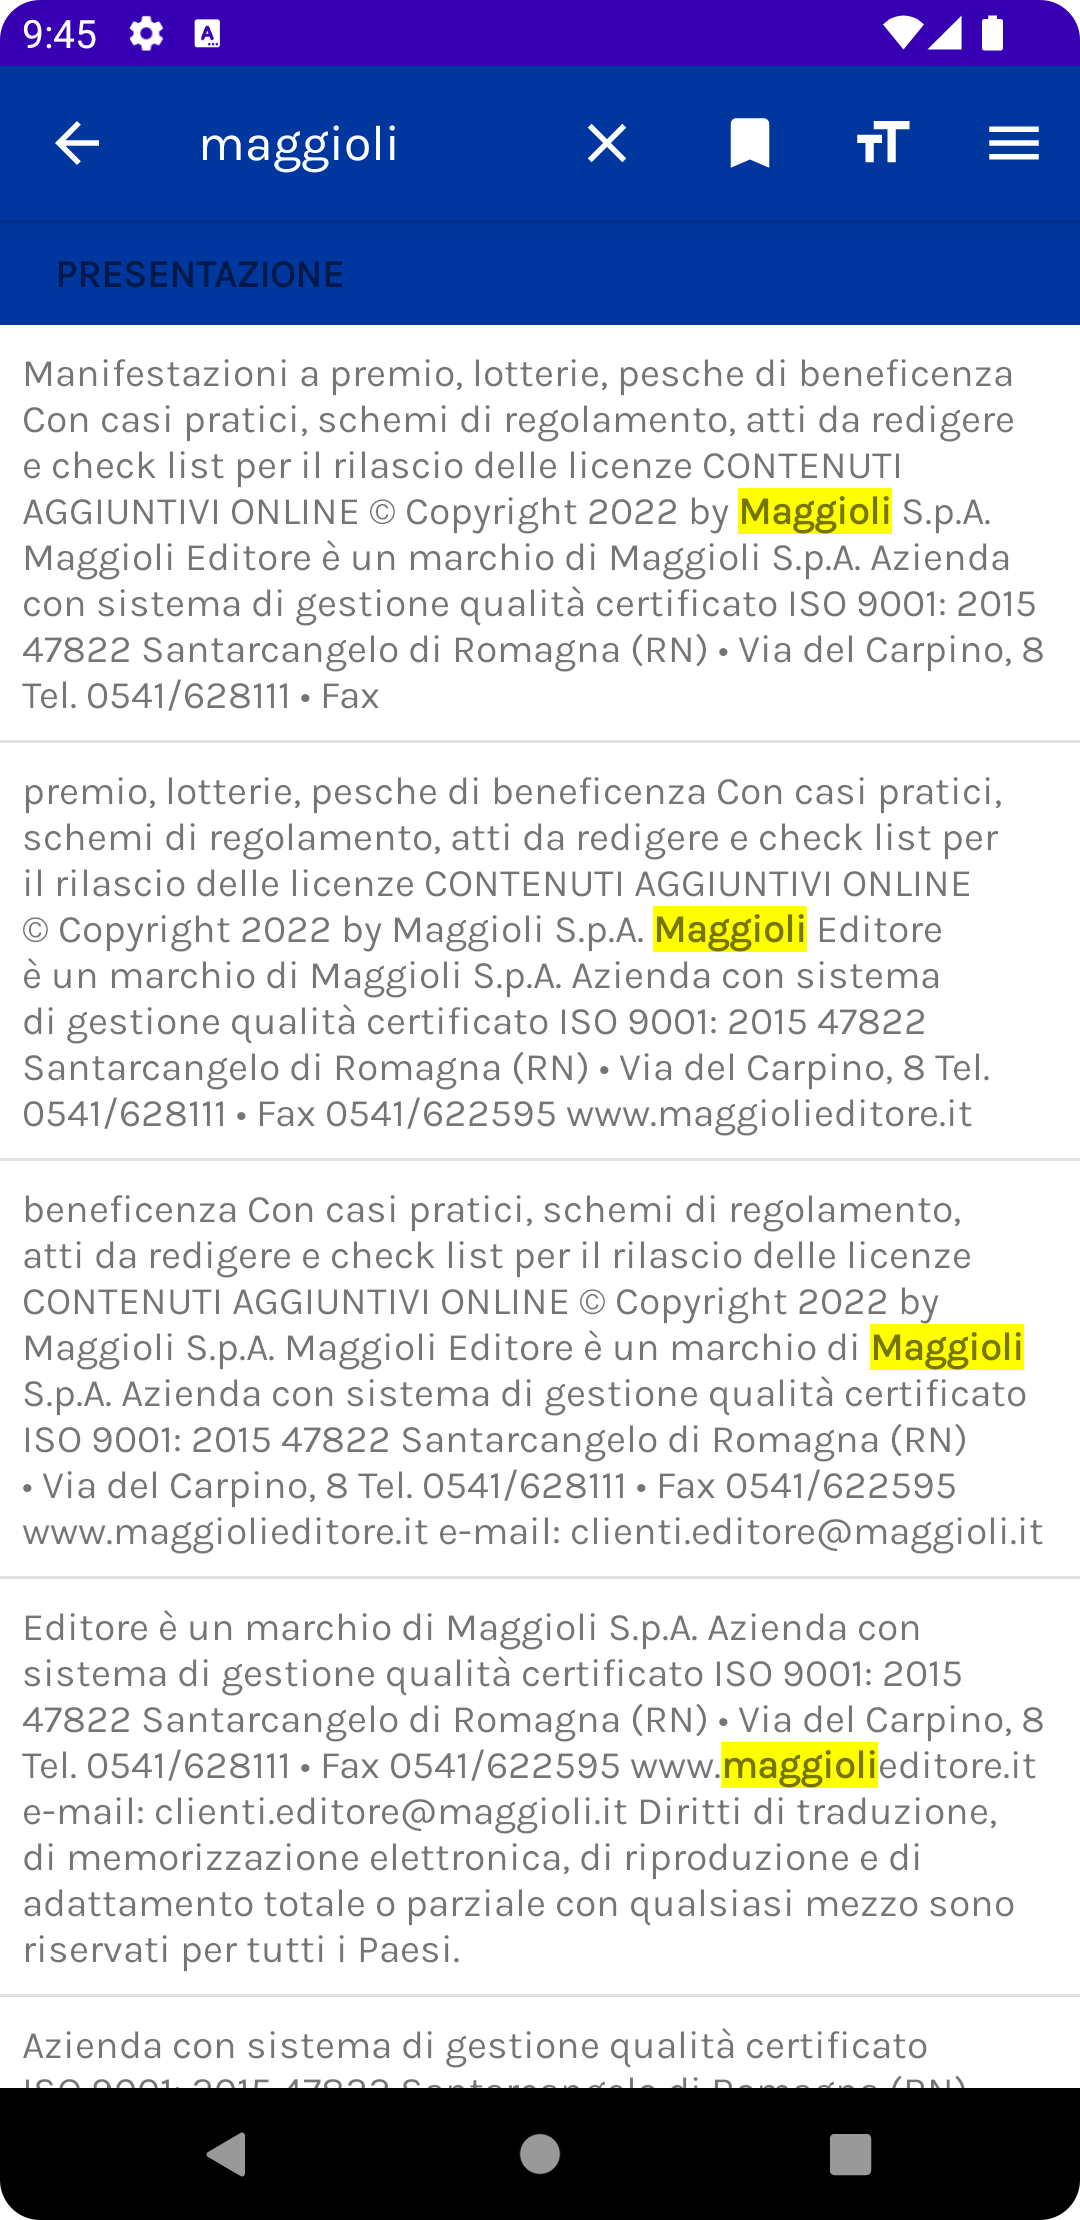
\includegraphics[width=0.2\textwidth]{ricerca_testo.png}
                \caption{Ricerca testuale nel contenuto del documento aperto con relativo risultato}
                \label{ricerca_testo}
            \end{figure}
            
            \begin{figure}[H]
                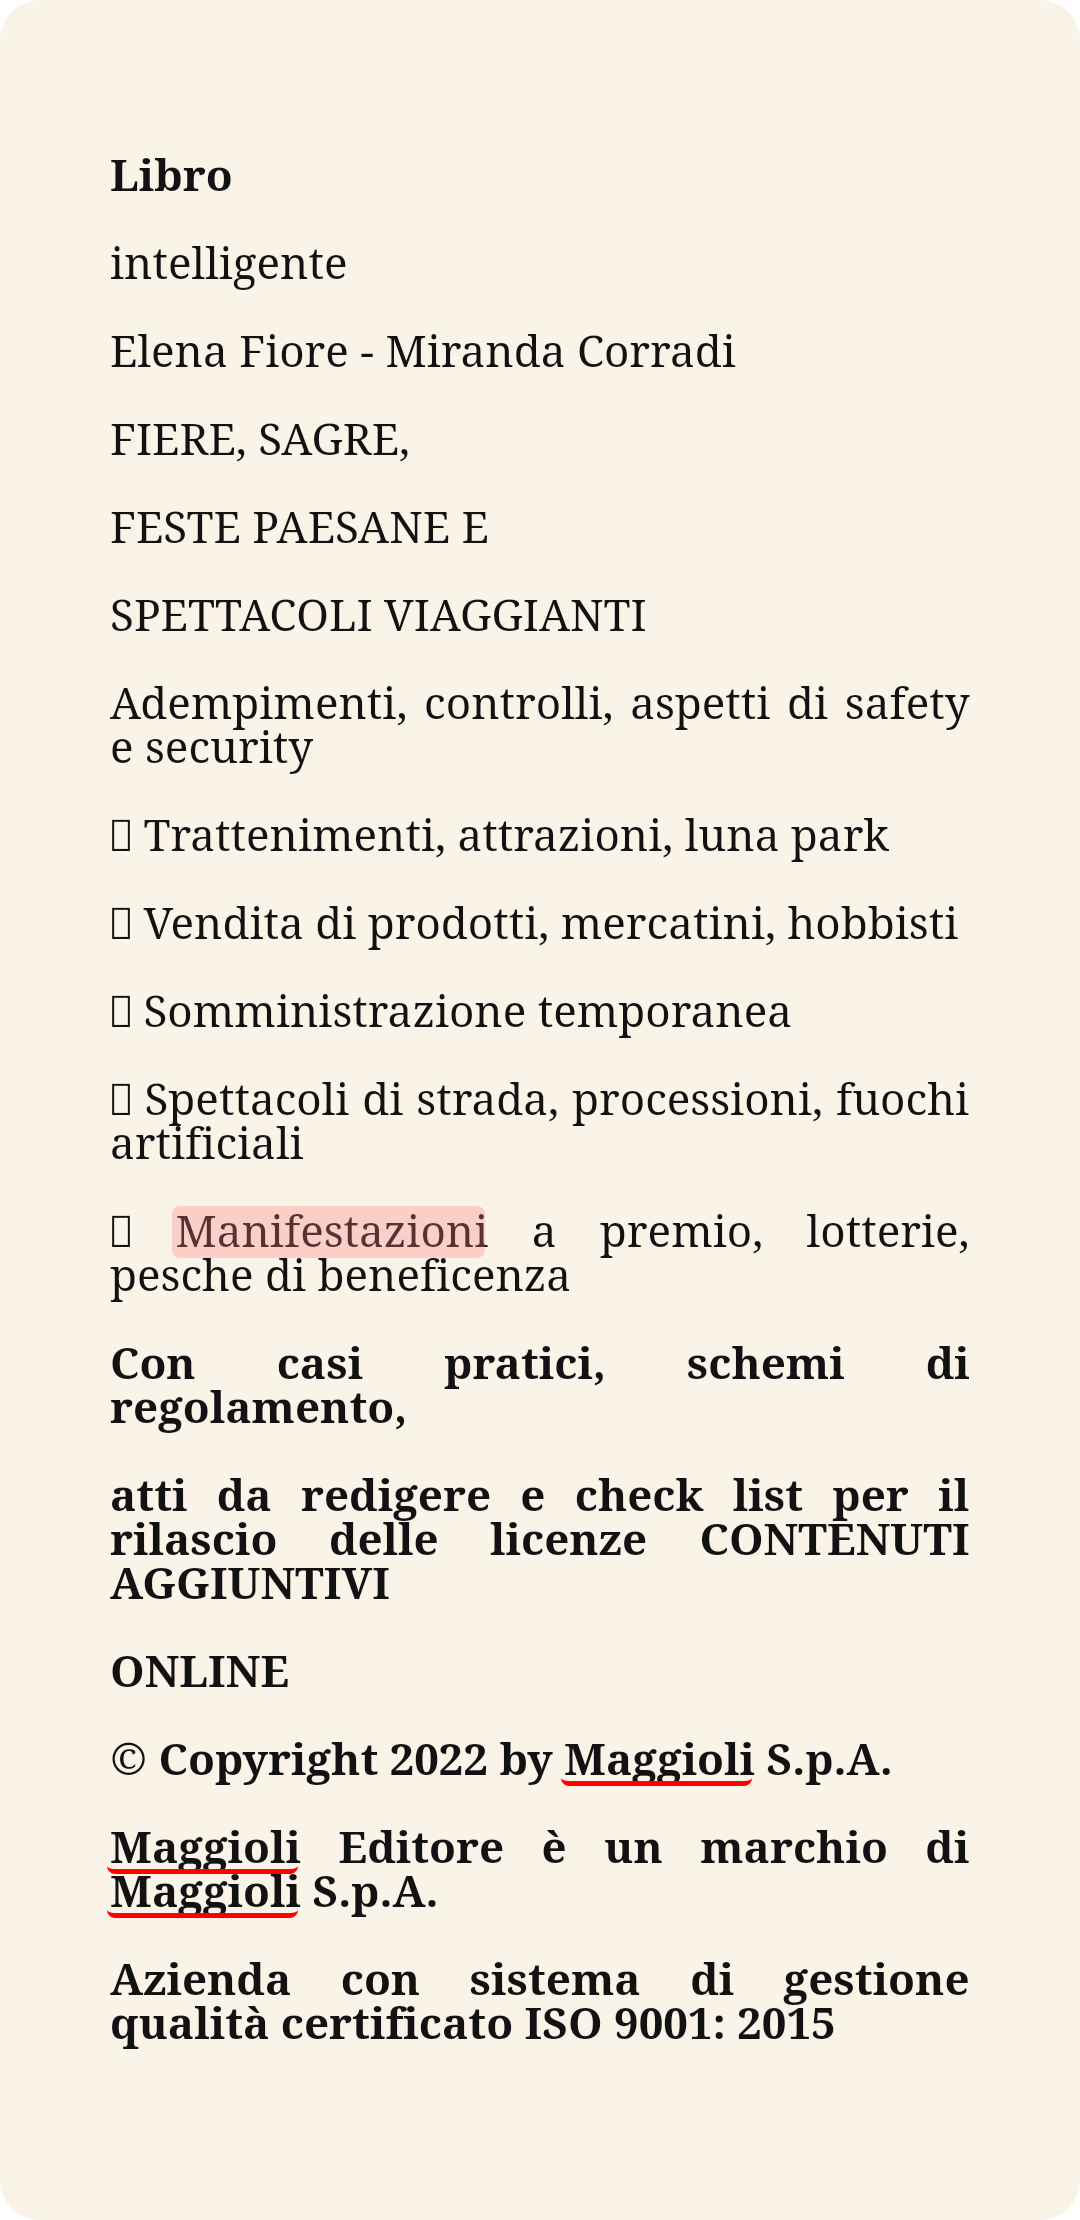
\includegraphics[width=0.2\textwidth]{ricerca_testo2.png}
                \caption{Evidenziazioni automatiche delle occorrenze del testo cercato}
                \label{ricerca_testo2}
            \end{figure}
        \end{multicols}
    \end{frame}

\end{document}
